
	\begin{frame}{Introduction}
		\begin{itemize}
			\pause
			\item Easy usage of MOAB Workload Manager and Dynamic Scheduler
			\pause
			\item Generate shell scripts for MOAB Workload Manager 
			\begin{itemize}
				\pause
				\item  send script via SSH to the bwUniCluster
			\end{itemize}
			\pause
			\item Visualization
			
		\end{itemize}
	\end{frame}
	
	\begin{frame}{Architecture}
		\begin{itemize}
	\pause
			\item Model-View-Presenter
			\begin{itemize}
				\pause
				\item FXML to describe the UI
				\pause
				\item Java code for application logic
			\end{itemize}
	        
				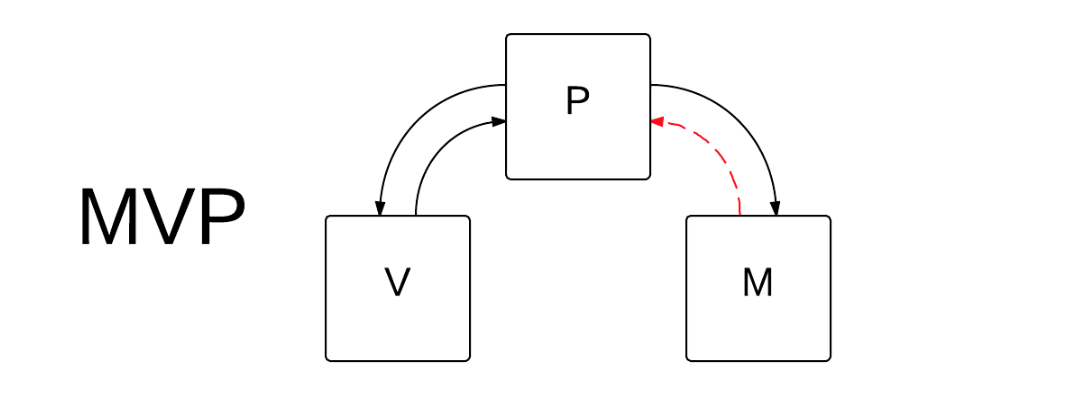
\includegraphics[width=300px, height=100px]{images/mvp.png}
		\end{itemize}
	\end{frame}
	
	
%	\subsection{Design}
%	\begin{frame}{Architecture (Design)}
%		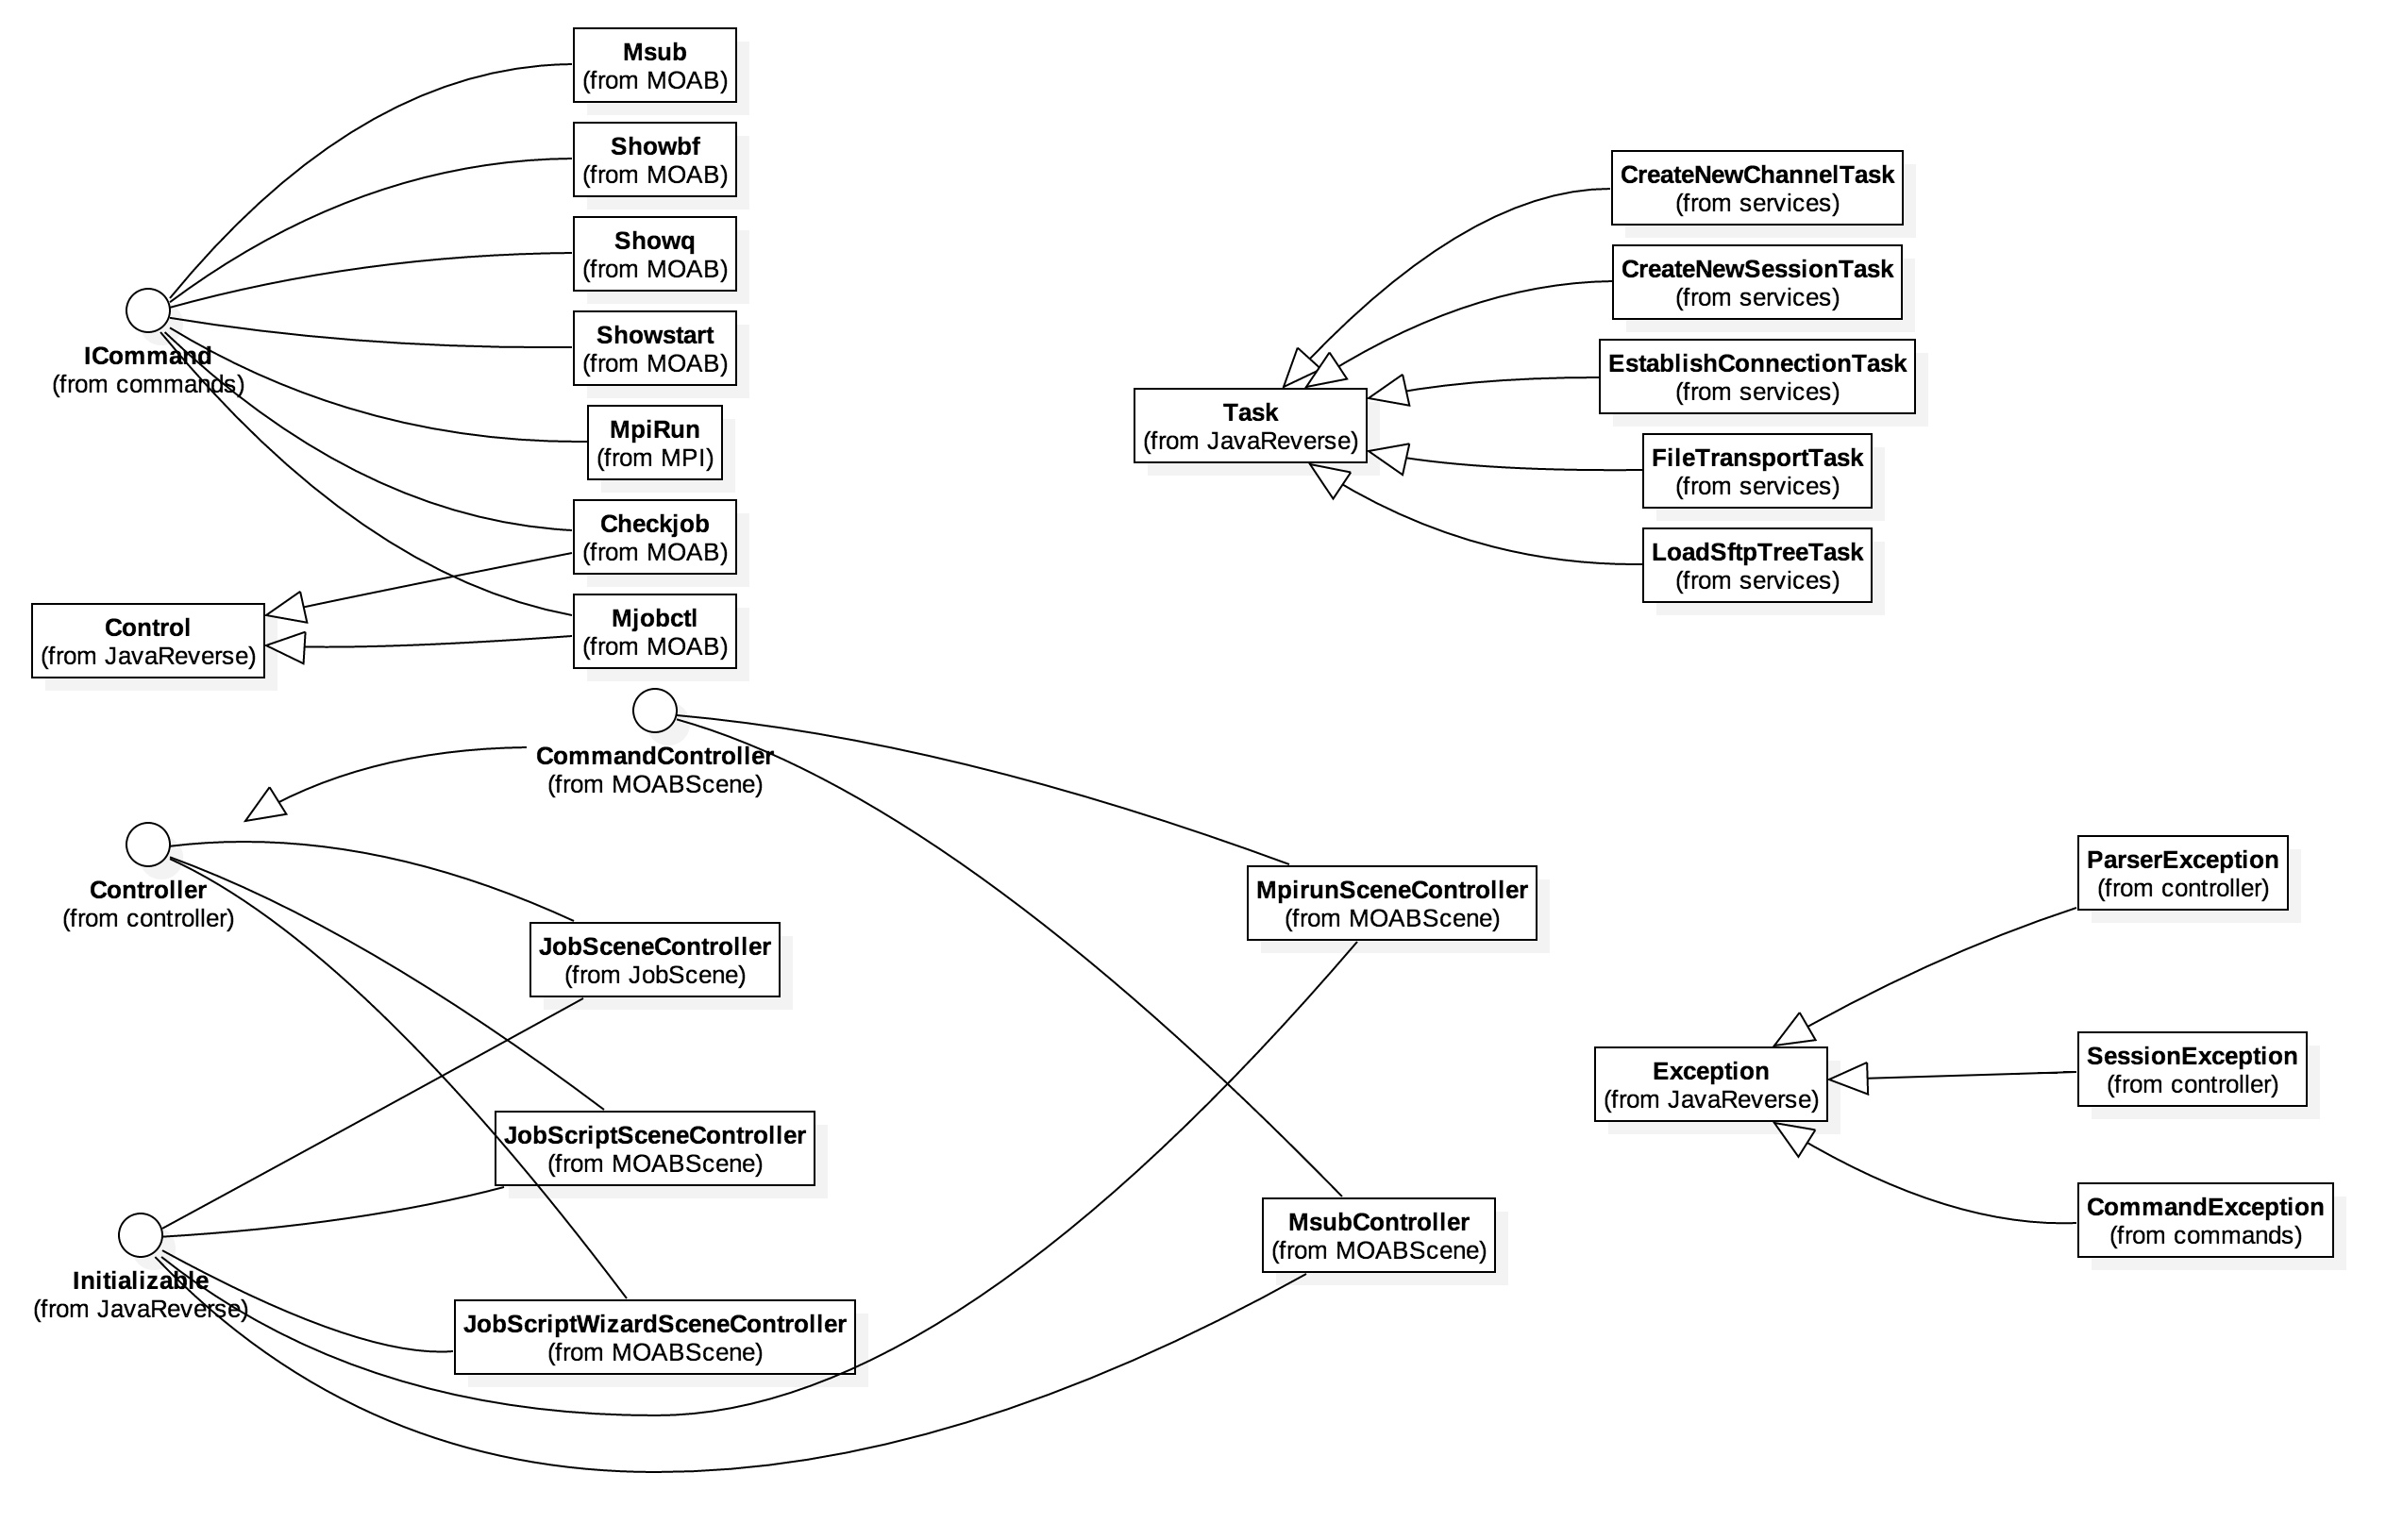
\includegraphics[width=300px, height=210px]{images/GUIDesign.png}
%	\end{frame}
	

	\begin{frame}{SSH-Connection}
		\begin{tikzpicture}[->,shorten >=1pt,auto,node distance=3cm,thick,main node/.style={ ellipse,draw,font=\sffamily\Large\bfseries}]
 
  \node[main node] (1) {Disconnected};
  \node[main node] (2) [below right of=1]{Connecting};
  \node[main node] (3) [below right of=2] {Ready};
  \node[main node] (4) [above right of=3] {Establishing};
  \node[main node] (5) [above right of=4] {Online};

  \path[every node/.style={font=\sffamily\small}]
    (1) edge [bend right] node[left] {Try Connection} (2)
        
    (2) edge [bend right] node[right] {Connection Failed} (1)
        edge [bend right] node[left] {Valid Connection} (3)
    (3) edge [bend left] node[right] {Initiate Connection} (4)
    		
    (4) edge [bend right] node[right] {Initiation Failed} (1)
       	edge [bend left] node[right] {Success} (5)
    (5)  edge [bend right] node[above] {Disconnect} (1)
         edge [bend left=90] node[right] {Offline} (3);
	\end{tikzpicture}
	\end{frame}
	
	\begin{frame}{Script Generator}
	\begin{itemize}
		\pause
		\item Shell script generator for MOAB Workload Manager:
		
		\begin{itemize}
			\pause
			\item parse msub command
			
			\pause			
			\item specify the directory in server using lazy tree 
			 
			\pause
			\item parse mpirun command
			
			\pause
			\item parse parameters of the dynamic scheduler
		\end{itemize}
			\end{itemize}
	\end{frame}
	
	
	
	\begin{frame}{Script Structure}
		
		\begin{block}{run\_scheduler.sh}
		        \#\#\#\# MOAB commands
		        \newline
		        \newline
				\#MSUB  -q develop\\
				\#MSUB  -l nodes=22:ppn=22\\
				\#MSUB  -l walltime=1000\\
				\#MSUB  -M uxdok@student.kit.edu
				\newline
				\newline
        				\#\#\#\# Directory
				\newline
				\newline
				cd ./Documents
				\newline
				\newline
        				\#\#\#\# MPI commands
        			\newline
        			\newline
				mpirun -np 4 ./myExec -design master-worker -strategy fifo
			
		\end{block}
	\end{frame}
	
	